\section{Main experimental results}
\label{sec:experiments}

This section presents our main experimental results in Image classification, detection and segmentation. We also include an ablation study. 
We refer the reader to the supplemental material for some additional hyper-parameter studies. 
Our code depend on the PyTorch~\cite{pytorch} and timm libraries~\cite{pytorchmodels}. We will share model weights along with a PyTorch implementation of our main models. 

\subsection{Classification results}
We first compare our model with competing approaches on the validation set of ImageNet1k (Imnet-val / Top-1) and ImageNet-v2 in Table~\ref{tab:mainres}. 
We report the compute requirement as reflected by FLOPs, the Peak memory usage, the number of parameters, and a throughput at inference time measured for a constant batch-size of 256 images.
%

We compare with various models, including classic models like ResNet-50 revisited with modern training recipes such as the one recently proposed by Wightman~\etal~\cite{wightman2021resnet}. 
Note however that different models may have received a different optimization effort, therefore the results on a single criterion are mostly indicative. That being pointed out, we believe that the \ournet results show that a simple columnar architecture is a viable choice compared to other attention-based approaches that are more difficult to optimize or scale.
%


\begin{figure}[t]
     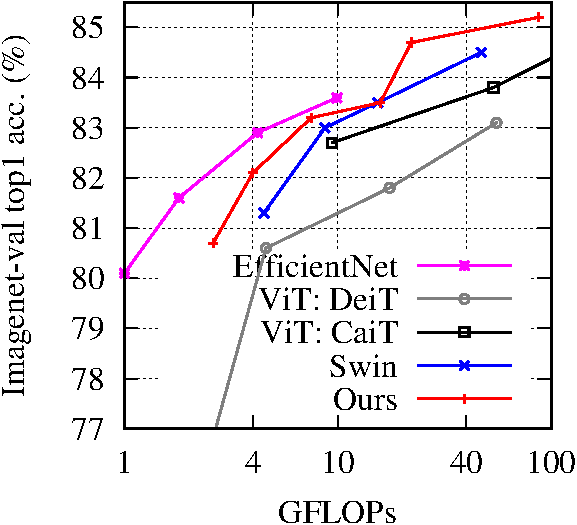
\includegraphics[height=0.5\linewidth,clip,trim=0 0 0 0pt]{figs/acc_vs_flops.pdf}\hfill
     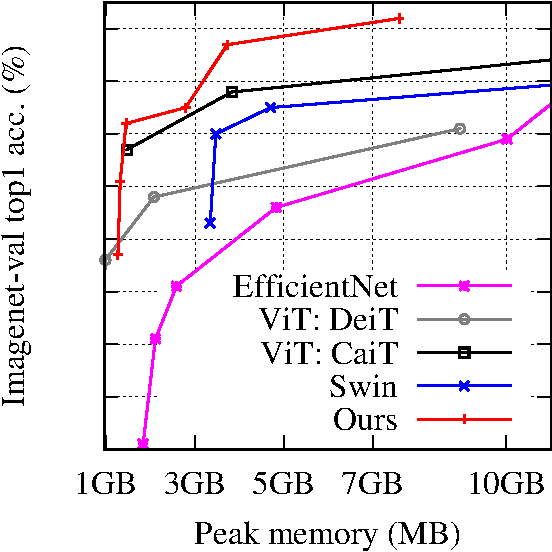
\includegraphics[height=0.5\linewidth,clip,trim=35 0 0 0pt]{figs/acc_vs_memory.pdf}
    \caption{\textbf{Trade-offs} for ImageNet-1k top 1 accuracy vs. FLOPs requirement and peak memory requirements (for a batch of 256 images). %
    Patch-based architectures are comparatively inferior w.r.t. the accuracy-FLOP trade-off than hierarchical ones, but offer better operating points in terms of the accuracy-memory compromise at inference time. 
    \label{fig:acc_flops_memory}}
\end{figure}



\begin{table}[t]

    \caption{
\textbf{Classification with Imagenet1k training.} 
We compare architectures with  based on convolutional networks, Transformers and feedforward networks with comparable FLOPs and number of parameters. All models are trained on ImageNet1k only without distillation nor self-supervised pre-training.
We report Top-1 accuracy on the validation set of ImageNet1k and ImageNet-V2 with different measure of complexity: throughput, FLOPs, number of parameters and peak memory usage. 
The throughput and peak memory are measured on a single V100-32GB GPU with batch size fixed to 256 and mixed precision. 
For ResNet~\cite{He2016ResNet} and RegNet~\cite{Radosavovic2020RegNet} we report the improved results from Wightman et al.~\cite{wightman2021resnet}. Note that different models may have received a different optimization effort. $\uparrow$R indicates that the model is fine-tuned at the resolution $R$. %
\label{tab:mainres}}
\vspace{-1ex}
    \centering
%
    \scalebox{0.66}{
    \begin{tabular}{@{\ }l@{}c@{\ \ }c@{\ \ \ }r@{\ \ }r|cc@{\ }}
        \toprule
        Architecture        & nb params & throughput & FLOPs & Peak Mem & Top-1  & V2 \\
                      & ($\times 10^6$) & (im/s) & ($\times 10^9$) & (MB)\ \ \ \  & Acc.  & Acc. \\[3pt]
\toprule
\multicolumn{7}{c}{\textbf{``Traditional'' ConvNets}} \\[3pt]
     ResNet-50~\cite{He2016ResNet,wightman2021resnet} &  25.6    & 2587  &  4.1      & 2182 & 80.4  & 68.7 \\
%
    \midrule
	 RegNetY-4GF~\cite{Radosavovic2020RegNet,wightman2021resnet}       & 20.6  & 1779  & \tzo4.0 & 3041 & 81.5  & 70.7 \\
	 RegNetY-8GF~\cite{Radosavovic2020RegNet,wightman2021resnet}       & 39.2  & 1158 & \tzo8.0 & 3939 & 82.2 & 71.1 \\
	 %
	 RegNetY-16GF~\cite{Radosavovic2020RegNet,Touvron2020TrainingDI}      & 83.6  & \pzo714 & \dzo16.0 & 5204   & 82.9  & 72.4 \\
	 %

    \midrule
% 
	 EfficientNet-B4~\cite{tan2019efficientnet} & 19.0  & \pzo573 & \tzo4.2 &  10006  & 82.9  & 72.3\\
	 EfficientNet-B5~\cite{tan2019efficientnet} & 30.0  & \pzo268 & \tzo9.9 &  11046  & 83.6  & 73.6\\
	 \midrule
	 NFNet-F0~\cite{Brock2021HighPerformanceLI} & 71.5 & \pzo950 & 12.4 & 4338 & 83.6  & 72.6 \\
	 NFNet-F1~\cite{Brock2021HighPerformanceLI} & 132.6\pzo & \pzo337 & 35.5 & 6628 & 84.7  & 74.4\\
%
\toprule
\multicolumn{7}{c}{\textbf{Vision Transformers and derivatives}} \\ [5pt]

% 
    ViT: DeiT-S~\cite{Touvron2020TrainingDI,wightman2021resnet}  & 22.0  & 1891 & \tzo4.6 & 987 & 80.6 &  69.4\\
	ViT: DeiT-B~\cite{Touvron2020TrainingDI}    & 86.6  & \pzo831  & \dzo17.5 & 2078 & 81.8 &  71.5\\
	%
	\midrule
	Swin-T-224~\cite{liu2021swin} & 28.3 & 1109 & 4.5 & 3345 & 81.3 &  69.5 \\
    Swin-S-224~\cite{liu2021swin} & 49.6 & \pzo718 & 8.7 & 3470 &  83.0 &   71.8 \\

    Swin-B-224~\cite{liu2021swin} & 87.8  & \pzo532 & 15.4 & 4695 & 83.5 &   \_ \\
%  
    \toprule
\multicolumn{7}{c}{\textbf{Vision MLP}} \\[3pt]
%    ResMLP-S12~\cite{Touvron2021ResMLPFN} &  15.0  & 3301 & \tzo3.0  & 755 &  76.6 &  64.4\\

    Mixer-L/16~\cite{tolstikhin2021MLPMixer} &  208.2\pzo &  322 & 44.6 &   2614 &   71.8 & 56.2  \\
    Mixer-B/16~\cite{tolstikhin2021MLPMixer} &  59.9 &   993 & 12.6  & 1448  &   76.4 &  63.2 \\
    ResMLP-S24~\cite{Touvron2021ResMLPFN} &  30.0  &  1681    & \tzo6.0  & 844 &  79.4 &  67.9 \\
    ResMLP-B24~\cite{Touvron2021ResMLPFN} &  116.0\pzo &      1120    & \dzo23.0 & 930  &   81.0 &  69.0 \\
    \toprule
    \multicolumn{7}{c}{\textbf{Patch-based ConvNets}} \\[3pt]
    ResMLP-S12 conv3x3~\cite{Touvron2021ResMLPFN} &  16.7  & 3217 & \tzo3.2  & 763 &  77.0  & 65.5\\
    ConvMixer-768/32~\cite{anonymous2022patches} & 21.1 & \pzo271 & 20.9 & 2644 & 80.2  & \_\\
    ConvMixer-1536/20~\cite{anonymous2022patches} & 51.6 & \pzo157 & 51.4 & 5312 & 81.4  & \_\\
    \midrule
%
    \rowcolor{Goldenrod}
    \ours-S60 & 25.2  & 1125 & 4.0 & 1321 & 82.1 &  71.0\\
    \rowcolor{Goldenrod}
    \ours-S120&  47.7 & \pzo580 & 7.5 & 1450 & 83.2 &  72.5\\
%
    \rowcolor{Goldenrod}
    \ours-B60 &  99.4 & \pzo541 & 15.8 & 2790 & 83.5 &   72.6\\
    \rowcolor{Goldenrod}
    \ours-B120 & 188.6\pzo  & \pzo280 & 29.9  & 3314 & 84.1 & 73.9\\
%
    \bottomrule
    \end{tabular}}
 % 
\end{table}

\paragraph{Higher-resolution.} 
There is a fine interplay between model size and resolution when it comes to the specific optimization of FLOPs and accuracy. We refer to the findings of Bello \etal~\cite{Bello2021RevisitingRI} who discussed some of these relationships, for instance the fact that small networks are better associated with smaller resolution. In our work we have not  optimized for the Pareto curve specifically. Since this trade-off is only one out of multiple criteria depending on the context, we prefer to report most of our results at the 224 and 384 resolutions. Table~\ref{tab:mainres} shows that our model significantly benefit from larger resolution images. See also Figures~\ref{fig:mem_vs_resolution_S60}  and \ref{fig:acc_vs_resolution_S60} where we analyze \ournet as a function of the image size. 
Table~\ref{tab:higher_res} we analyze \ournet pre-trained on ImageNet21k with different fine-tuning resolution. All network are pre-trained on ImageNet21k during 90 epochs at resolution $224\times 224$, finetune on ImageNet1k at resolution $384\times 384$ and then fine-tune at bigger resolution. 
 
\begin{table}[t]
    \centering
    \caption{\textbf{ImageNet21k pre-training:} Comparison of \ournet fine-tuned at different resolutions on ImageNet1k. We report peak memory (MB) and throughput (im/s) on one GPU V100 with batch size 256 and mixed precision. Larger resolution provides classification improvement with the same model, but significantly increase the resource requirements.  
    [\emph{italic refers to a few results obtained with a longer training}]. 
    }
    \vspace{-1ex}
    \scalebox{0.7}{
    \begin{tabular}{cccccc}
    \toprule
         Model & GFLOPs & Peak Mem & throughput & Res & Imnet-val Acc  \\
         \midrule
         S60   &   \pzo\pzo4.0      &   \pzo1322        &    1129      &  224  & \phantom{[{\emph{83.3}}]} 82.9 [{\emph{83.5}}]  \\
         S60   &     \pzo\pzo6.6    &    \pzo2091       &    \pzo692      &  288  & \phantom{[{\emph{84.2}}]} 84.0 [{\emph{84.4}}]  \\
         S60   & \pzo11.8    & \pzo3604  & \pzo388  &  384 & \phantom{[\emph{85.0}]} 84.6 [{\emph{84.9}}] \\
%
%
         S60   & \pzo20.9    & \pzo6296  & \pzo216 &  512 & \phantom{[{\emph{85.4}}]} 85.0 [{\emph{85.4}}]\\
        %

         %
         \midrule
         B60   &   \pzo15.8      &  \pzo2794        &    \pzo547      &  224  &  \phantom{[{\emph{85.0}}]} 85.0 [{\emph{85.4}}]  \\
         B60   &   \pzo26.1      &   \pzo4235        &    \pzo328      &  288  & 85.7  \\
         B60   & \pzo46.5    & \pzo7067  & \pzo185 &  384 &  \phantom{[{\emph{86.5}}]} 86.1   [{\emph{86.5}}]\\

         \midrule 
         L60   &   \pzo28.1      &   \pzo3913        &     \pzo394     &  224  &  85.6  \\
         L60   &   \pzo46.4      &    \pzo5801       &    \pzo237      &  288  &  86.1  \\
         L60   &   \pzo82.5      &    \pzo9506       &   \pzo132       &  384  &  86.4  \\
         \midrule
         B120   &  \pzo29.8       &   \pzo3313        &     \pzo280     & 224  & 86.0    \\
         B120   &   \pzo49.3      &    \pzo4752       &     \pzo169     & 288  & 86.6    \\
         B120   &  \pzo87.7   & \pzo7587  & \pzo\pzo96 &  384 & 86.9   \\

         \midrule 
         L120   &   \pzo53.0      &    \pzo4805       &    \pzo204      &  224  &  86.1  \\
         L120   &    \pzo87.5     &    \pzo6693       &    \pzo123      &  288  &  86.6  \\
         L120   &    155.5     &      10409     &    \pzo\pzo68      &  384  &  87.1  \\
        
         \bottomrule
    \end{tabular}
    \label{tab:higher_res}}
\end{table}


\subsection{Segmentation results and detection}

%

\paragraph{Semantic segmentation}
We evaluate our models with semantic segmentation experiments on the ADE20k dataset~\cite{Zhou2017ScenePT}.
This dataset consist in 20k training and 5k validation images with labels over 150 categories. 
For the training, we adopt the same schedule as in Swin~\cite{liu2021swin}:~160k iterations with UpperNet~\cite{Xiao2018UnifiedPP}. 
At test time we evaluate with a single scale similarly to XciT~\cite{el2021xcit} and multi-scale as in Swin~\cite{liu2021swin}.
As our approach is not pyramidal we only use the final output of our network in UpperNet. 
Unlike concurrent approaches we only use the output of our network at different levels in UpperNet which simplifies the approach.

Our results are reported in Table~\ref{tab:sem_seg}.
We can observe that our approach although simpler is at the same level as the state-of-the-art Swin architecture~\cite{liu2021swin} and outperforms XCiT~\cite{el2021xcit} in terms of FLOPs-mIoU tradeoff.


\begin{table}[t]

       \caption{\textbf{ADE20k semantic segmentation} performance using UperNet \cite{xiao2018unified} (in comparable settings). All models are pre-trained on ImageNet1k except models with $^\dagger$ symbol that are pre-trained on ImageNet21k. 
       \label{tab:sem_seg}}
           \vspace{-1ex}
        \centering
        \scalebox{0.7}{
        \begin{tabular}{lcccc}
        \toprule
             \multirow{2}{*}{Backbone} & \multicolumn{4}{c}{UperNet}  \\
             & \#params & FLOPs & Single scale & Multi-scale  \\
             \cmidrule{2-3}
             \cmidrule{4-5}
             & ($\times 10^6$) & ($\times 10^9$) & mIoU  & mIoU \\
            \midrule 
             ResNet50 \cite{He2016ResNet} & 66.5 & \_ & 42.0 & \_ \\
             DeiT-S \cite{Touvron2020TrainingDI} & 52.0 & 1099 & \_ & 44.0 \\
             XciT-T12/16 \cite{el2021xcit} & 34.2 & \pzo874  & 41.5  & \_\\
             XciT-S12/16 \cite{el2021xcit}  & 54.2  & \pzo966 & 45.9 & \_\\
             Swin-T  \cite{liu2021swin} & 59.9 & \pzo945 & 44.5 & 46.1 \\

             \rowcolor{Goldenrod}
             \ours-S60 & 57.1 & \pzo952 & \textbf{46.0}  & \textbf{46.9}\\

            \midrule
             XciT-M24/16 \cite{el2021xcit} & 112.2 & 1213 & 47.6 & \_ \\
             XciT-M24/8 \cite{el2021xcit} & 110.0 & 2161  & 48.4 & \_ \\
             Swin-B \cite{liu2021swin} & 121.0 & 1188  & 48.1 & 49.7 \\

            \rowcolor{Goldenrod}
            \ours-B60 & 140.6 & 1258  & 48.1  & 48.6 \\

              \rowcolor{Goldenrod}
             \ours-B120 & 229.8 & 1550  & \textbf{49.4}  & \textbf{50.3}\\
            \midrule 
            Swin-B$^\dagger$ ($640\times 640$) & 121.0 & 1841  & 50.0 & 51.6 \\
            CSWin-B$^\dagger$~\cite{Dong2021CSWinTA} & 109.2 & 1941  & 51.8 & 52.6 \\
            

            
             \rowcolor{Goldenrod}
             \ours-S60$^\dagger$ & \pzo57.1 & \pzo952 & 48.4  & 49.3 \\
            \rowcolor{Goldenrod}
            \ours-B60$^\dagger$ & 140.6 & 1258  & 50.5  & 51.1 \\
            \rowcolor{Goldenrod}
             \ours-B120$^\dagger$ & 229.8 & 1550  & 51.9  & 52.8  \\

            \rowcolor{Goldenrod}
             \ours-L120$^\dagger$ & 383.7 & 2086  &  \textbf{52.2} & \textbf{52.9}   \\

        \bottomrule     
        \end{tabular}
        } 
\end{table}

\paragraph{Detection \& instance segmentation}

We have evaluated our models on detection and instance segmentation tasks on COCO~\cite{Lin2014MicrosoftCC}. 
We adopt the Mask R-CNN~\cite{he2017mask} setup with the commonly used $\times 3$ schedule.
Similar to segmentation experiments, as our approach is not pyramidal, we only use the final output of our network in Mask R-CNN~\cite{he2017mask}. 
Our results are in Table~\ref{tab:coco_det}.
We can observe that our simple approach is on par with state of the art architecture like  Swin~\cite{liu2021swin} and XCiT~\cite{el2021xcit} in terms of FLOPs-AP tradeoff.

\begin{table}[t]
        \captionof{table}{\footnotesize \textbf{COCO object detection and instance segmentation} performance on the mini-val set. All backbones are pre-trained on ImageNet1k, use Mask R-CNN model~\cite{he2017mask} and are trained with the same 3$\times$ schedule. 
        %
        }%
            \vspace{-1ex}
        \centering
        \scalebox{0.72}{
        \begin{tabular}{l@{\ \ }r c@{\ \ } | c@{\ \ \ }c@{\ \ }c|c@{\ \ }c@{\ \ } c}
        \toprule
             Backbone & \!\!\!\ \#params\!\!\! & \!\!\!GFLOPs\ \!\!\! & $\text{AP}^{b}$ & $\text{AP}^{b}_{50}$ & $\text{AP}^{b}_{75}$ & $\text{AP}^{m}$ & $\text{AP}^{m}_{50}$ & $\text{AP}^{m}_{75}$\\ 
            \midrule 
            ResNet50 \cite{He2016ResNet} & 44.2M & 180 & 41.0 & 61.7 & 44.9 & 37.1 & 58.4 & 40.1 \\
            ResNet101 \cite{He2016ResNet} & 63.2M & 260 & 42.8 & 63.2 & 47.1 & 38.5 & 60.1 & 41.3 \\
            ResNeXt101-64 \cite{xie2017aggregated} & \!101.9M\! & 424 & 44.4 & 64.9 & 48.8 & 39.7 & 61.9 & 42.6 \\
            \midrule
            
            PVT-Small \cite{wang2021pyramid} & 44.1M & \_  & 43.0 & 65.3 & 46.9 & 39.9 & 62.5 & 42.8 \\
            PVT-Medium \cite{wang2021pyramid} & 63.9M & \_ & 44.2 & 66.0 & 48.2 & 40.5 & 63.1 & 43.5 \\


            XCiT-S12/16 & 44.4M & 295 & 45.3 & 67.0 & 49.5 & 40.8 & 64.0 & 43.8  \\
            XCiT-S24/16 \cite{el2021xcit} & 65.8M & 385  & 46.5 & 68.0 & 50.9 & 41.8 & 65.2  & 45.0 \\

            ViL-Small \cite{zhang2021multi} & 45.0M & 218 & 43.4 & 64.9 & 47.0 & 39.6 & 62.1 & 42.4 \\
            ViL-Medium \cite{zhang2021multi} & 60.1M & 294 & 44.6 & 66.3 & 48.5 & 40.7 & 63.8 & 43.7 \\
            ViL-Base \cite{zhang2021multi}  & 76.1M & 365 & 45.7 & 67.2 & 49.9 & 41.3 & 64.4 & 44.5 \\

            Swin-T \cite{liu2021swin} & 47.8M & 267 & 46.0 & 68.1  & 50.3 & 41.6 & 65.1 & 44.9 \\

          
           \rowcolor{Goldenrod}
            \ours-S60 & 44.9M  & 264 &  46.4 & 67.8 & 50.8 & 41.3 & 64.8 &44.2 \\
            \rowcolor{Goldenrod}
            \ours-S120 & 67.4M &  339 & 47.0 & 69.0  & 51.4 & 41.9 & 65.6 & 44.7\\
        \bottomrule     
     \end{tabular}     
     } % 
     \label{tab:coco_det}
\end{table}



\subsection{Ablations}

All our ablation have been carried out with ``Seed 0'', i.e., we report only one result without handpicking. For this reason one must keep in mind that there is a bit of noise in the performance measurements: On ImageNet1k-val, we have measured with the seeds 1 to 10 a standard deviation of $\pm 0.11\%$ in top-1 accuracy for a S60 model, which concurs with measurements done on ResNet-50 trained with modern training procedures~\cite{wightman2021resnet}. 

\paragraph{Stochastic depth.} Our main parameter is the stochastic depth, whose effect is analyzed in Fig. \ref{fig:stochastic_depth}. This regularization slows down the training, yet with long enough schedules, higher values of the \textit{drop-path} hyperparameter lead to better performance at convergence.  
We train with the values reported in Table~\ref{tab:layernorm_vs_batchnorm}. When fine-tuning at higher resolutions or from ImageNet21k, we reduce this \textit{drop-path} by 0.1. 
See also Appendix~\ref{sec:apdx_explo} for a preliminary ablation on the learning rate and weight decay, which showed that the performance is relatively stable with respect to these parameters. Fixing this hyper-parameter couple is possibly suboptimal but makes it convenient and more resource-efficient to adjust a single hyper-parameter per model. Therefore, we have adopted this choice in all our experiments. 
%


\begin{figure}
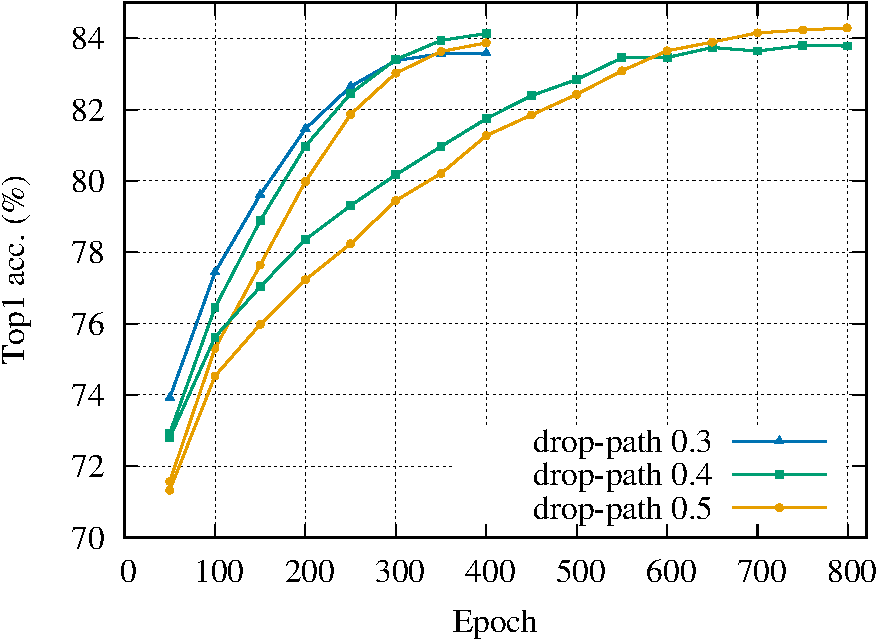
\includegraphics[width=\linewidth]{figs/stochastic_depth_vs_epoch.pdf}
\caption{Effect of stochastic depth on the performance for  varying training duration for a \ournet-B120 model trained @ resolution 224. 
The corresponding hyper-parameter (\textit{drop-path}) is selected among 0.3, 0.4 or 0.5 in that case, which means that we randomly drop up to half of the layers. Smaller values of the drop-rate converge more rapidly but saturate. 
\label{fig:stochastic_depth}} 
\end{figure}


\paragraph{Architectural ablation.} 
In Table~\ref{tab:ablation_archi}, we have conducted various ablations of our architecture with the S60 model.
We compare the impact of class attention \textit{vs.} average-pooling. Average-pooling is the most common aggregation strategy in ConvNet while class attention is only used with transformers~\cite{touvron2021going}. 
We compare also convolutional stem \textit{vs.} linear projection for the patch extraction in the image, 
LayerNorm \textit{vs.} BatchNorm and 
Multi-heads class attention as used in CaiT~\cite{touvron2021going} \textit{vs.} single-head class attention. Our single-head design reduces the memory consumption and simplifies attention map visualization.



%


\begin{table}[t]
%
\caption{Ablation of our model: we modify each time a single architectural characteristic in our \ournet model S60, and measure how it affects the classification performance on ImageNet1k. Batch-normalization improves the performance a bit. The convolutional stem is key for best performance, and the class-attention brings a slight improvement in addition to enabling attention-based visualisation properties. 
\label{tab:ablation_archi}}
\vspace{-0.5ex}
\centering
\scalebox{0.8}{
     %
    \begin{tabular}{rclr}
    \toprule
    \multicolumn{3}{l}{$\downarrow$ Modification to the architecture} & Top-1 acc. \\
    \midrule
    \rowcolor{blue!5} 
    none    &  & &   82.1   \\
    class-attention       & $\rightarrow$ & average pooling  & 81.9\\ 
    conv-stem             & $\rightarrow$ & linear projection & 80.0 \\ 
    layer-normalization   & $\rightarrow$ & batch-normalization & 82.4 \\ 
    single-head attention & $\rightarrow$ & multi-head attention & 81.9 \\ 
    a single class-token  & $\rightarrow$ & one class-token per class & 81.1 \\ 
% 
    \bottomrule 
    \end{tabular}}
\end{table}

\paragraph{Attention-based pooling with ConvNets.}

Interestingly, our learned aggregation stage increases the performance of a very competitive ResNet model. When adopting the recent training recipe from Wightman \etal~\cite{wightman2021resnet}, % 
we obtain $80.1\%$ top-1 accuracy on Imagenet1k by adding a learned pooling to a ResNet50. This is an improvement of $+0.3\%$ to the corresponding 300-epoch baseline based on average pooling. 
%
The class attention  only slightly increases the number of FLOPs of the models:
4.6B vs 4.1B. %

We point out that we have not optimized the training recipes further (either without or with class-attention). This result is reported for a single run (Seed 0) in both cases. 


\paragraph{Patch pre-processing.} 
In the vanilla patch-based approaches as vision transformers~\cite{dosovitskiy2020image,Touvron2020TrainingDI} and MLP-style models~\cite{tolstikhin2021MLPMixer,Touvron2021ResMLPFN}, the images patches are embedded by one linear layer.
Recent works~\cite{graham2021levit,Xiao2021EarlyCH} show that replacing this linear patch pre-processing by a few convolutional layers allows to have a more stable architecture~\cite{Xiao2021EarlyCH} with better performance.
So, in our work we choose to use a convolutional stem instead of pure linear projection.
We provide in Table~\ref{tab:ablation_archi} an ablation of this component.








